\documentclass[11pt,a4paper]{article}
\usepackage{amsmath}\usepackage{amssymb}\usepackage[table]{xcolor}
\usepackage{tabularx}\usepackage{multirow}\usepackage{geometry}
\usepackage{enumitem}\usepackage{parskip}\usepackage{titlesec}
\usepackage{tocloft}\usepackage[most]{tcolorbox}
\usepackage{tikz}\usepackage{pgfplots}\pgfplotsset{compat=1.18}\usetikzlibrary{arrows.meta,calc,positioning,shapes.geometric,patterns}
\geometry{margin=2.5cm}
\titleformat{\section}{\large\bfseries}{}{0em}{}
\setlength{\cftbeforesecskip}{6pt}
\definecolor{q1color}{HTML}{D6EAF8}\definecolor{q2color}{HTML}{D5F5E3}
\definecolor{q3color}{HTML}{FDEBD0}\definecolor{q4color}{HTML}{F9E79F}
\definecolor{q5color}{HTML}{E8DAEF}\definecolor{q6color}{HTML}{FADBD8}
\definecolor{q7color}{HTML}{D1F2EB}\definecolor{q8color}{HTML}{FCF3CF}
\definecolor{q9color}{HTML}{EBDEF0}\definecolor{q10color}{HTML}{F5EEF8}
\newenvironment{mstab}[1]{%
  {\color{#1!75!black}\nobreak Mark Scheme}\par\nopagebreak\smallskip
  \arrayrulecolor{#1!70!black}\renewcommand{\arraystretch}{1.3}%
  \tabularx{\textwidth}{|>{\columncolor{#1!12}\raggedright\arraybackslash}p{1.9cm}|>{\columncolor{#1!12}}X|>{\columncolor{#1!12}\centering\arraybackslash}p{1.1cm}|}%
  \hline\rowcolor{#1!45} Question & Answer & Marks \\ \hline}{%
  \endtabularx\arrayrulecolor{black}\par\medskip}
\newtcolorbox{ansbox}[1]{colback=#1!8,colbacktitle=#1!30,colframe=#1!70!black,coltitle=black,fonttitle=\normalfont,title=Worked Solution,boxrule=0.6pt,arc=2mm,left=4pt,right=4pt,top=4pt,bottom=4pt,breakable}
\newcommand{\topiclabel}[1]{\hfill\normalfont\small\itshape\textcolor{black!55}{#1}}
\newcommand{\examq}[4]{\section[#1 - Q#2]{#1 - Q#2 - #3 - #4}}
\begin{document}
\begin{center}
  {\LARGE \textbf{Cambridge O Level Physics 5054/22/M/J/16}}\\[6pt]
  {\large May/June 2016 -- Mark Scheme \& Worked Solutions}
\end{center}
\bigskip

%=================================================================
\examq{5054/22/M/J/16}{1}{Motion or Kinematics \textperiodcentered\ Forces or Dynamics}{5}

\begin{mstab}{q1color}
1(a) & mark at a time between 4.0 and 7.5 seconds & B1 \\ \hline
 & $(a =)\ (v - u)/t$ numerical or algebraic\newline or $(a =)$ gradient of graph stated & C1 \\ \cline{2-3}
\multirow{-2}{1.9cm}{1(b)} & $2.5\ \mathrm{m/s^2}$ & A1 \\ \hline
 & forward force and backward force clear & B1 \\ \cline{2-3}
\multirow{-2}{1.9cm}{1(c)} & equal forces (in horizontal direction)\newline or no resultant force\newline or forces cancel\,/\,balance\,/\,in equilibrium & B1 \\ \hline
\end{mstab}

\begin{ansbox}{q1color}
For (a), ``deceleration'' means the graph is \emph{falling}, and ``non-uniform'' means its \emph{gradient is changing} -- so you need a point on a part of the line that is both sloping downwards and curved. The straight sloping section of Fig.\,1.1 is where the deceleration is uniform; beyond it the line bends as the car levels out. Mark and label any point on that curved falling part: \textbf{any time between $4.0$\,s and $7.5$\,s} is accepted. A suitable point, at $t = 5.0$\,s, is marked below.
\begin{center}
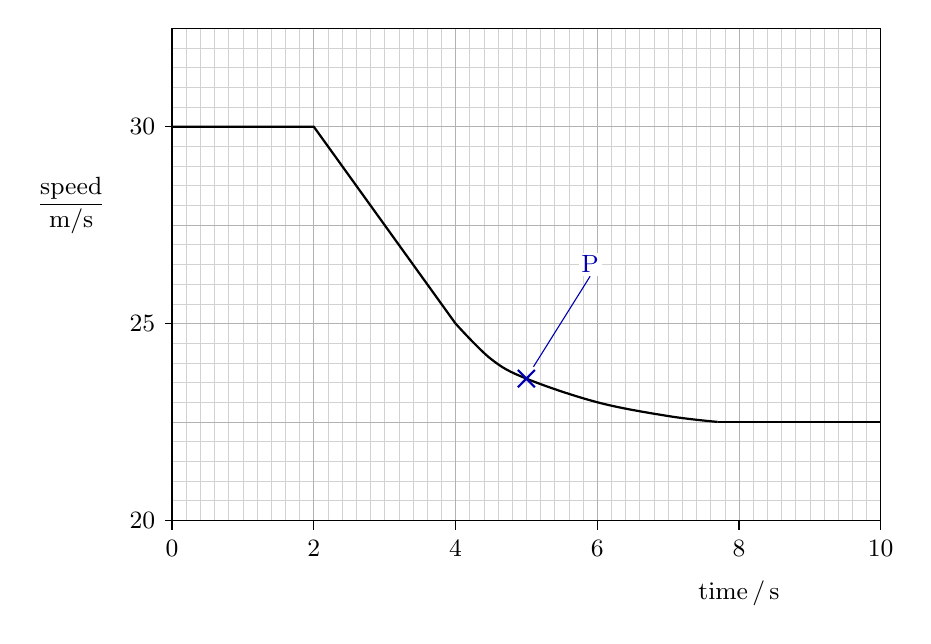
\begin{tikzpicture}[>=Stealth, font=\small, x=0.9cm, y=0.5cm]
  \fill[white] (0,0) rectangle (10,12.5);
  \draw[gray!35, very thin, xstep=0.2, ystep=0.5] (0,0) grid (10,12.5);
  \draw[gray!60, very thin, xstep=2, ystep=2.5] (0,0) grid (10,12.5);
  \draw (0,0) rectangle (10,12.5);
  \foreach \x in {0,2,...,10} \draw (\x,0) -- (\x,-0.25) node[below] {\x};
  \foreach \v/\l in {0/20,5/25,10/30} \draw (0,\v) -- (-0.1,\v) node[left] {\l};
  \node[below] at (8,-1.3) {time\,/\,s};
  \node[anchor=east] at (-0.8,8) {$\dfrac{\text{speed}}{\text{m/s}}$};
  % given speed-time graph (speed axis starts at 20 m/s)
  \draw[thick] (0,10) -- (2,10) -- (4,5);
  \draw[thick] plot[smooth, tension=0.6] coordinates {(4,5) (4.5,4.1) (5,3.6) (6,3.0) (7,2.65) (7.7,2.5)};
  \draw[thick] (7.7,2.5) -- (10,2.5);
  % answer: a point on the curved falling part
  \draw[blue!70!black, thick] (5,3.6) +(-0.12,-0.22) -- +(0.12,0.22) (5,3.6) +(-0.12,0.22) -- +(0.12,-0.22);
  \draw[blue!70!black] (5.1,3.9) -- (5.9,6.2) node[above, fill=white, inner sep=1pt] {P};
\end{tikzpicture}
\end{center}

For (b), deceleration is the \textbf{gradient of the speed--time graph}, so take two points on the \emph{straight} sloping section that contains $t = 3.0$\,s. Reading Fig.\,1.1, the speed falls from $30$\,m\,/\,s at $t = 2.0$\,s to $25$\,m\,/\,s at $t = 4.0$\,s, so
\[ a = \frac{v - u}{t} = \frac{25 - 30}{4.0 - 2.0} = -2.5\ \mathrm{m/s^2}, \]
i.e.\ a \textbf{deceleration of $2.5\ \mathrm{m/s^2}$}. The minus sign only records that the car is slowing; a deceleration is quoted as a positive number. Note that you must use the straight part alone -- averaging over the whole $0$--$10$\,s would mix in the constant-speed section and the curve, and would not give the value \emph{at} $t = 3.0$\,s.

For (c), at $t = 1.0$\,s the graph is \textbf{horizontal}: the speed is constant, so the acceleration is zero. By Newton's first law, zero acceleration means \textbf{zero resultant force}. Two horizontal forces act on the car: the \textbf{forward driving force} delivered to the road by the driven wheels, and the \textbf{backward resistive force} (air resistance together with friction). Since the resultant of these two is zero, they must be \textbf{equal in magnitude and opposite in direction} -- they balance, or cancel, so the car is in equilibrium and travels at constant speed.
\end{ansbox}

%=================================================================
\examq{5054/22/M/J/16}{2}{Work Energy and Power}{6}

\begin{mstab}{q2color}
 & $(PE =)\ mgh$ or $Fd$ or $5 \times 3.5$ & C1 \\ \cline{2-3}
\multirow{-2}{1.9cm}{2(a)} & 17.5\,J or 17\,J or 18\,J & A1 \\ \hline
2(b)(i) & (efficiency $=$ useful) energy output\,/\,energy input\newline in any form but all three quantities must be mentioned if efficiency is not the subject of the equation & B1 \\ \hline
 & $17.5/0.65$ or $17.5/65$\newline or $0.65/65 = $ (a)\,/\,energy input & C1 \\ \cline{2-3}
\multirow{-2}{1.9cm}{2(b)(ii)} & 26.9\,J or 27\,J & A1 \\ \hline
2(c) & due to friction (in bearings of motor)\newline or due to (electrical) resistance (in motor)\newline or air resistance acts\newline or thermal energy\,/\,heat produced\,/\,lost (in resistance of motor\,/\,due to friction) & B1 \\ \hline
\end{mstab}

\begin{ansbox}{q2color}
For (a), the gain in gravitational potential energy is $\Delta E_p = mgh$, but here the \emph{weight} is given rather than the mass, and $mg$ \emph{is} the weight. So use work done against gravity $= Fd = \text{weight} \times \text{height}$:
\[ \Delta E_p = 5.0 \times 3.5 = 17.5\ \mathrm{J}. \]
(Rounded answers of $17$\,J or $18$\,J are accepted.) Because the load rises at \emph{constant speed} its kinetic energy does not change, so all the useful work done by the motor goes into potential energy.

For (b)(i), efficiency compares what you want with what you paid for:
\[ \text{efficiency} = \frac{\text{useful energy output}}{\text{energy input}} \qquad \left(\times 100\% \text{ for a percentage}\right). \]
All three quantities must appear; if you write it rearranged, say as $\text{energy input} \times \text{efficiency} = \text{useful energy output}$, that is also acceptable.

For (b)(ii), the useful energy output is the $17.5$\,J of potential energy from (a), and the efficiency is $0.65$, so
\[ \text{energy input} = \frac{\text{useful energy output}}{\text{efficiency}} = \frac{17.5}{0.65} = 26.92 \approx 26.9\ \mathrm{J}\ (27\ \mathrm{J}). \]
Check the sense of the answer: the input must be \emph{larger} than the useful output, and $26.9 > 17.5$, so the division is the right way round. (Dividing by $65$ instead of $0.65$ and then correcting by a factor of $100$ is equally acceptable.)

For (c), the missing $26.9 - 17.5 = 9.4$\,J has not vanished -- it has been transferred to the surroundings as \textbf{thermal energy (and a little sound)} instead of becoming potential energy of the load. Any one cause is enough: \textbf{friction} in the bearings of the motor and in the pulley, \textbf{electrical resistance} of the motor windings (which dissipates $I^2R$ as heat), or \textbf{air resistance} on the moving parts and load. No real machine is $100\%$ efficient for exactly this reason.
\end{ansbox}

%=================================================================
\examq{5054/22/M/J/16}{3}{Deformation \textperiodcentered\ Mass Weight and Density}{5}

\begin{mstab}{q3color}
3(a)(i) & C & M1 \\ \hline
3(a)(ii) & data quoted to prove stretches more at end\newline or extensions\,/\,changes in length increase\,/\,are not the same (at higher loads) & A1 \\ \hline
3(a)(iii) & 4.5\,cm & B1 \\ \hline
 & (tie rock to spring A)\newline $\bullet$ find weight\,/\,force\,/\,newtons using length or extension and graph or match readings (in table)\newline $\bullet$ find known weight\,/\,mass\,/\,force\,/\,N that gives same extension of spring\newline $\bullet$ use of proportionality with length or extension\newline $\bullet$ extension (in cm)\,/\,1.6 & B1 \\ \cline{2-3}
\multirow{-2}{1.9cm}{3(b)} & (mass $=$) weight\,/\,$g$\newline or weight\,/\,gravitational field (strength) & B1 \\ \hline
\end{mstab}

\begin{ansbox}{q3color}
For (a)(i), the limit of proportionality is where extension stops being directly proportional to load, so look for the spring whose \emph{equal} load steps stop producing \emph{equal} length increases. That spring is \textbf{C}.

For (a)(ii), you must quote the numbers from Fig.\,3.1 rather than just assert it. Every load step in the table is the same, $0.5$\,N, so for proportionality each step must add the same length. For spring C the successive increases in length are
\[ 10.5 - 9.7 = 0.8, \quad 11.3 - 10.5 = 0.8, \quad 13.1 - 11.3 = 1.8, \quad 16.9 - 13.1 = 3.8\ \mathrm{cm}. \]
The first two steps add $0.8$\,cm each, but the last two add $1.8$\,cm and then $3.8$\,cm -- so \textbf{the extensions get bigger at higher loads} and C is no longer obeying the straight-line relationship. (For comparison, spring A adds $0.8$\,cm for \emph{every} step and spring B about $0.9$\,cm for every step, so both are still proportional throughout.)

For (a)(iii), spring A gains $0.8$\,cm for each $0.5$\,N, i.e.\ $1.6$\,cm per newton. At a load of $1.0$\,N its length is $6.1$\,cm, and the extension produced by that $1.0$\,N is $1.0 \times 1.6 = 1.6$\,cm. So the unstretched (natural) length is
\[ l_0 = 6.1 - 1.6 = 4.5\ \mathrm{cm}. \]
Any other row gives the same answer -- e.g.\ at $3.0$\,N, $9.3 - 3.0 \times 1.6 = 9.3 - 4.8 = 4.5$\,cm -- which is a good check.

For (b), two steps are needed, and the mark scheme awards one for each. \textbf{First find the rock's weight.} Hang the rock on spring A, measure the new length $l$, and get the extension $e = l - 4.5$\,cm. Spring A is proportional with $1.6$\,cm per newton, so
\[ \text{weight} = \frac{e\ (\mathrm{in\ cm})}{1.6}\ \mathrm{N}. \]
(Equivalently: read the weight off a graph of the table's data, or simply find which known weight produces that same extension.) \textbf{Then convert weight to mass} using $W = mg$:
\[ m = \frac{W}{g} = \frac{\text{weight}}{10}\ \mathrm{kg}. \]
A spring measures \emph{weight} (a force), not mass, so this last division by the gravitational field strength is essential.
\end{ansbox}

%=================================================================
\examq{5054/22/M/J/16}{4}{Thermal Properties \& Temperature \textperiodcentered\ Kinetic Model of Matter}{6}

\begin{mstab}{q4color}
4(a) & steam\newline or (water) vapour\newline or water in gaseous form & B1 \\ \hline
 & $(E =)\ mL$ numerical or algebraic\newline or $52\,000 - 6000$ or $46\,000$\,(J) seen & C1 \\ \cline{2-3}
 & $(52\,000 - 6000)/20$ or $46\,000/20$ & C1 \\ \cline{2-3}
\multirow{-3}{1.9cm}{4(b)} & 2300\,J\,/\,g or $2.3 \times 10^{6}$\,J\,/\,kg & A1 \\ \hline
 & fast moving\,/\,energetic molecules escape\,/\,evaporate\,/\,break bonds\,/\,become gas & B1 \\ \cline{2-3}
\multirow{-2}{1.9cm}{4(c)} & leaving slow(er) molecules\,/\,less energetic molecules\newline or reducing average (kinetic) energy (of molecules or liquid) & B1 \\ \hline
\end{mstab}

\begin{ansbox}{q4color}
For (a), the bubbles form \emph{within} the liquid once it reaches its boiling point, so they are bubbles of the water's own vapour: \textbf{steam (water vapour)}, i.e.\ water in the gaseous state. They are not air -- any dissolved air was driven off long before the water reached $100\,^{\circ}$C, and the water has been boiling for a long time.

For (b), first work out how much of the supplied energy actually went into vaporising water. Of the $52\,000$\,J supplied, $6000$\,J leaked away to the atmosphere, so
\[ E = 52\,000 - 6000 = 46\,000\ \mathrm{J} \]
was used to turn liquid into vapour. (Note that the water is \emph{boiling steadily}, so its temperature is constant and none of this energy goes into raising the temperature -- it all goes into the latent heat.) The mass vaporised is the mass lost from the beaker, $20$\,g. From $E = mL$,
\[ L = \frac{E}{m} = \frac{46\,000}{20} = 2300\ \mathrm{J\,/\,g}. \]
In SI units that is $2300\ \mathrm{J/g} \times 1000\ \mathrm{g/kg} = 2.3 \times 10^{6}$\,J\,/\,kg, which is the accepted value for the specific latent heat of vaporisation of water.

For (c), the key idea is that the molecules in a liquid do \emph{not} all have the same speed -- there is a spread of molecular kinetic energies. Evaporation happens at the surface, and only the \textbf{fastest, most energetic molecules} there have enough energy to \textbf{break the bonds} holding them in the liquid and escape into the air above. Because it is always the most energetic molecules that leave, the molecules \textbf{left behind are the slower, less energetic ones}, so the \textbf{average kinetic energy of the remaining liquid falls}. Temperature is a measure of that average molecular kinetic energy, so the temperature of the water drops -- the water cools. (The escaping molecules also carry their energy away with them, which is the same statement seen from outside.)
\end{ansbox}

%=================================================================
\examq{5054/22/M/J/16}{5}{Light (Reflection/Refraction/Lenses)}{6}

\begin{mstab}{q5color}
5(a)(i) & long-sight or far-sight or hypermetropia & B1 \\ \hline
5(a)(ii) & rays do not come together (on back of eye)\newline or rays do not converge (on retina)\newline or it\,/\,the image is not formed on retina\,/\,back of eye\newline or it\,/\,the image is formed behind retina\,/\,back of eye & B1 \\ \hline
5(b)(i) & lens between rays and eyeball \textbf{and} a converging lens shown & B1 \\ \hline
5(b)(ii) & converging or convex & B1 \\ \hline
\end{mstab}

\begin{ansbox}{q5color}
For (a)(i), read the symptom carefully: distant objects are seen clearly but \emph{near} objects are blurred. That is \textbf{long sight} (far sight, or \emph{hypermetropia}). The opposite defect, short sight, would blur the distant objects instead.

For (a)(ii), a sharp image needs all the rays from one point on the object to be brought back together at one point \emph{on the retina}. Rays from a \emph{near} object arrive at the eye strongly diverging, so they need a lot of converging. In a long-sighted eye the lens is too weak (or the eyeball too short), so the rays are \textbf{not converged enough}: in Fig.\,5.1 they \textbf{do not come together on the back of the eye}. If you continued them they would meet \emph{behind} the retina. The retina therefore receives a spread-out patch of light instead of a point, and the image looks blurred.

For (b)(i), the correction must do the converging that the eye cannot do. Draw a \textbf{converging (biconvex) lens in front of the eyeball}, between the incoming rays and the eye -- symmetrically fat in the middle and thin at the edges. Then continue each of the three rays: at the lens each one bends \emph{towards} the principal axis, and the three now meet at a single point \textbf{on the retina} at the back of the eye. The extra convergence provided by the spectacle lens makes up exactly the amount the eye's own lens is short of. The lens and the completed rays are shown below.
\begin{center}
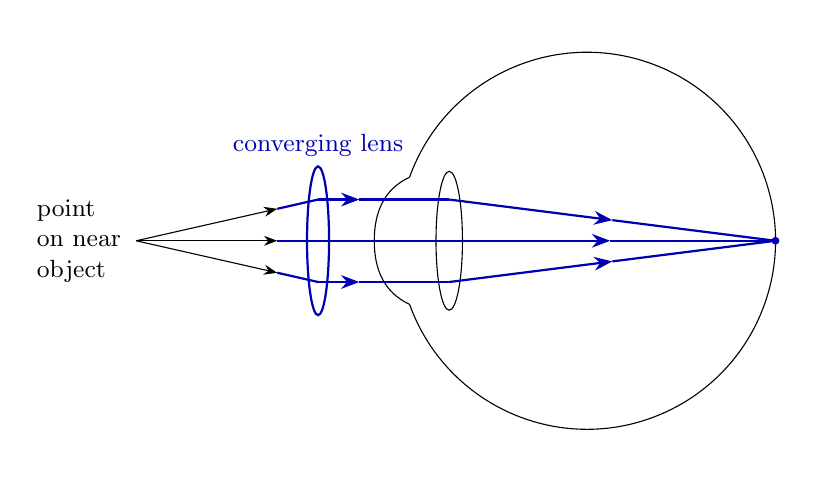
\begin{tikzpicture}[>=Stealth, font=\small, scale=0.7]
  % eyeball, cornea and eye lens (given)
  \draw (8.18,0) ++(160.3:3.42) arc[start angle=160.3, end angle=-160.3, radius=3.42];
  \draw (4.96,1.153) to[out=205,in=90] (4.32,0) to[out=-90,in=155] (4.96,-1.153);
  \draw (5.68,0) ellipse (0.24 and 1.26);
  % given rays from the point on the near object
  \node[align=left, anchor=east] at (-0.1,0) {point\\on near\\object};
  \foreach \y in {0.58,0,-0.58} \draw[->] (0,0) -- (2.56,\y);
  % answer: converging lens in front of the eye
  \draw[blue!70!black, thick] (3.3,0) ellipse (0.2 and 1.35);
  \node[blue!70!black, above] at (3.3,1.35) {converging lens};
  % answer: rays continued, meeting on the retina
  \foreach \s in {1,-1} {
    \draw[blue!70!black, thick] (2.56,0.58*\s) -- (3.3,0.748*\s);
    \draw[blue!70!black, thick, ->] (3.3,0.748*\s) -- (4.05,0.748*\s);
    \draw[blue!70!black, thick] (4.05,0.748*\s) -- (5.68,0.748*\s);
    \draw[blue!70!black, thick, ->] (5.68,0.748*\s) -- (8.64,0.374*\s);
    \draw[blue!70!black, thick] (8.64,0.374*\s) -- (11.6,0);
  }
  \draw[blue!70!black, thick, ->] (2.56,0) -- (8.6,0);
  \draw[blue!70!black, thick] (8.6,0) -- (11.6,0);
  \fill[blue!70!black] (11.6,0) circle (2pt);
\end{tikzpicture}
\end{center}

For (b)(ii), the lens needed is therefore a \textbf{converging (convex) lens}. A positive-power lens adds convergence; a diverging (concave) lens would do the opposite and would be the correction for short sight.
\end{ansbox}

%=================================================================
\examq{5054/22/M/J/16}{6}{Electromagnetic Spectrum}{6}

\begin{mstab}{q6color}
6(a)(i) & red & B1 \\ \hline
6(a)(ii) & blue & B1 \\ \hline
6(b) & ANY 2 from (the use must agree with the type)\newline \textbf{Microwaves} -- B1\newline use -- satellite television, telephone, mobile\,/\,cell phones; cooking, heating in a microwave oven, television remote, radar, communication -- B1\newline \textbf{X(-rays)} -- B1\newline use -- hospital use in medical imaging or security imaging, killing cancerous cells, and engineering applications such as detecting cracks in metal, crystallography -- B1\newline \textbf{gamma (rays)} -- B1\newline use -- medical treatment in killing cancerous cells, and engineering applications such as detecting cracks in metal, sterilisation, tracer applications, radiotherapy -- B1 & B4 \\ \hline
\end{mstab}

\begin{ansbox}{q6color}
For (a)(i), within the visible spectrum the wavelength decreases steadily as you go from red through to violet, so of the colours listed in Fig.\,6.1 the \textbf{largest wavelength} belongs to \textbf{red} -- the colour nearest the infra-red end.

For (a)(ii), all electromagnetic waves travel at the same speed $c$ in a vacuum, and $c = f\lambda$, so frequency and wavelength are \emph{inversely} related: the shortest wavelength has the highest frequency. Of the five colours shown, the shortest wavelength is \textbf{blue} (the colour nearest the ultra-violet end), so blue has the \textbf{highest frequency}.

For (b), the question has already used up visible light, infra-red, ultra-violet and radio waves, so the remaining components of the spectrum to choose from are \textbf{microwaves}, \textbf{X-rays} and \textbf{gamma rays}. Name any \textbf{two} and give one use of each -- and the use must match the component you named, since one mark is for the name and one for the use.

\begin{itemize}[nosep,leftmargin=*]
\item \textbf{Microwaves} -- satellite television and satellite telephone links, mobile (cell) phone communication, radar, television remote controls, and cooking or heating food in a microwave oven (the waves are absorbed by water molecules in the food).
\item \textbf{X-rays} -- medical imaging of bones and teeth, security scanning of baggage, killing cancerous cells, crystallography, and engineering uses such as detecting cracks in metal castings.
\item \textbf{Gamma rays} -- radiotherapy to kill cancerous cells, sterilising medical instruments and food, medical tracers, and again detecting cracks in metals.
\end{itemize}

Note that ``killing cancer cells'' and ``detecting cracks in metal'' are allowed for either X-rays or gamma rays, but the two uses you give must be \emph{different} from each other.
\end{ansbox}

%=================================================================
\examq{5054/22/M/J/16}{7}{Electric Charge}{6}

\begin{mstab}{q7color}
7(a) & any insulator, e.g.\ perspex, plastic, nylon, rubber & B1 \\ \hline
 & top of P shows a net negative charge with some negative charges under rod & B1 \\ \cline{2-3}
\multirow{-2}{1.9cm}{7(b)} & bottom of P has equal number of positive charges & B1 \\ \hline
7(c)(i) & clear net negative charge on P\newline and (net) negative charges above or at middle line & B1 \\ \hline
7(c)(ii)1 & negative (charges)\,/\,electrons flow to earth\newline or (P) becomes neutral & B1 \\ \hline
7(c)(ii)2 & charges spread over P & B1 \\ \hline
\end{mstab}

\begin{ansbox}{q7color}
For (a), an electrical insulator has no free charges to carry a current, so almost any non-metal will do: \textbf{perspex, plastic, nylon or rubber} (polythene, glass, dry wood and air are also insulators). Avoid naming a metal, and avoid ``wood'' without ``dry'', since damp wood conducts.

For (b), this is \textbf{charging (or rather polarising) by induction}. Metal P contains free electrons. The positively charged rod held just above P attracts those free electrons, which drift towards the rod and collect on the \emph{upper} surface of P. So draw the \textbf{top of P with a net negative charge}, with the negative signs concentrated in the region \textbf{directly under the rod}. P as a whole is still uncharged -- nothing has been added or removed -- so the electrons that moved up have left behind an \textbf{equal number of positive charges, drawn along the bottom of P}. The two amounts must look equal, because the total charge on P is still zero. The charges are shown in blue below.
\begin{center}
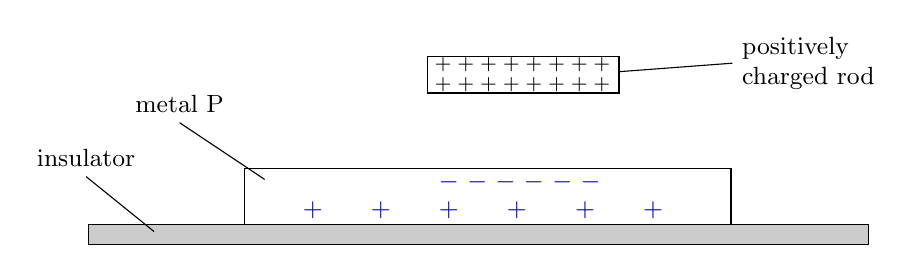
\begin{tikzpicture}[>=Stealth, font=\small, scale=0.72]
  % insulator, metal P and the positively charged rod (given)
  \fill[gray!40] (-2.75,-0.35) rectangle (11.0,0);
  \draw (-2.75,-0.35) rectangle (11.0,0);
  \draw (0,0) -- (0,1) -- (8.575,1) -- (8.575,0);
  \draw (3.225,2.325) rectangle (6.6,2.975);
  \foreach \y in {2.47,2.83} \foreach \x in {3.5,3.9,...,6.4} \node[inner sep=0pt] at (\x,\y) {\scriptsize $+$};
  \draw (6.6,2.7) -- (8.6,2.85) node[right, align=left] {positively\\charged rod};
  \draw (0.35,0.8) -- (-1.15,1.8) node[above] {metal P};
  \draw (-1.6,-0.12) -- (-2.8,0.85) node[above] {insulator};
  % answer: electrons drawn to the top under the rod, equal positive charge left at the bottom
  \foreach \x in {3.6,4.1,...,6.1} \node[blue!70!black, inner sep=0pt] at (\x,0.75) {$-$};
  \foreach \x in {1.2,2.4,...,7.2} \node[blue!70!black, inner sep=0pt] at (\x,0.25) {$+$};
\end{tikzpicture}
\end{center}

For (c)(i), the earth wire gives the charges a route to an effectively infinite reservoir. The rod is still attracting electrons, and now more electrons can be \textbf{drawn up from earth onto P}. So P acquires a \textbf{clear net negative charge}: show noticeably more negative signs than positive ones, with the \textbf{negative charges reaching above or at least to the middle line} of P rather than hugging the top surface. The charges are shown in blue below.
\begin{center}
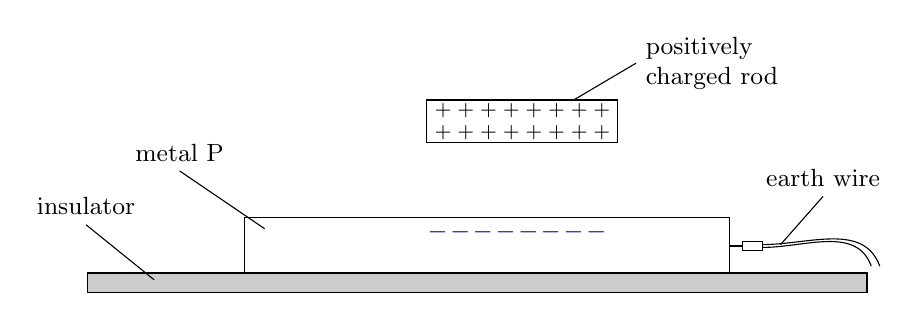
\begin{tikzpicture}[>=Stealth, font=\small, scale=0.72]
  % insulator, metal P, earth wire and the positively charged rod (given)
  \fill[gray!40] (-2.775,-0.35) rectangle (10.975,0);
  \draw (-2.775,-0.35) rectangle (10.975,0);
  \draw (0,0) -- (0,0.975) -- (8.55,0.975) -- (8.55,0);
  \draw (8.55,0.475) -- (8.775,0.475);
  \draw (8.775,0.4) rectangle (9.125,0.55);
  \draw (9.125,0.5) to[out=0,in=110] (11.2,0.12);
  \draw (9.125,0.45) to[out=0,in=110] (11.05,0.12);
  \draw (3.2,2.3) rectangle (6.575,3.05);
  \foreach \y in {2.48,2.87} \foreach \x in {3.5,3.9,...,6.4} \node[inner sep=0pt] at (\x,\y) {\scriptsize $+$};
  \draw (5.8,3.05) -- (6.9,3.7) node[right, align=left] {positively\\charged rod};
  \draw (9.45,0.5) -- (10.2,1.35) node[above] {earth wire};
  \draw (0.35,0.78) -- (-1.15,1.8) node[above] {metal P};
  \draw (-1.6,-0.12) -- (-2.8,0.85) node[above] {insulator};
  % answer: only negative charge, in the top half of P under the rod
  \foreach \x in {3.4,3.8,...,6.3} \node[blue!70!black, inner sep=0pt] at (\x,0.72) {$-$};
\end{tikzpicture}
\end{center}

For (c)(ii)1, with the earth wire \emph{still connected}, removing the rod removes the attraction that was holding the extra electrons on P. They repel one another and are free to leave, so the \textbf{excess electrons flow back down the wire to earth} and \textbf{P returns to being neutral} -- it ends up uncharged.

For (c)(ii)2, if the earth wire is \emph{disconnected first}, the extra electrons are trapped on P: there is no longer any path to earth. P is therefore left with a permanent negative charge. When the rod is then taken away, nothing holds those electrons at the top any more, so they repel one another and simply \textbf{spread out over the whole of P} -- P is left uniformly negatively charged. This is how a conductor is charged \emph{negatively} using a \emph{positive} rod, and it is why the order of the two operations matters so much.
\end{ansbox}

%=================================================================
\examq{5054/22/M/J/16}{8}{Electro Magnetism / Electromagnetic Induction \textperiodcentered\ Electric Circuits}{5}

\begin{mstab}{q8color}
 & current\,/\,a.c.\ (in primary coil) creates magnetic field\newline or current\,/\,a.c.\ magnetises iron & B1 \\ \cline{2-3}
\multirow{-2}{1.9cm}{8(a)} & changing magnetic field (in secondary) & B1 \\ \hline
8(b) & it\,/\,secondary has less turns (than primary)\newline or primary has more turns (than secondary)\newline or (some) flux escapes & B1 \\ \hline
8(c) & (steel is) a permanent magnet\newline or weaker fields produced\newline or (steel) difficult to magnetise\,/\,demagnetise\newline or (steel) is a hard magnetic material & B1 \\ \hline
8(d) & passes current\,/\,charge in one direction\newline or has high resistance\,/\,is an insulator when current in one direction\,/\,reverse biased & B1 \\ \hline
\end{mstab}

\begin{ansbox}{q8color}
For (a), build the chain of cause and effect in two steps -- one mark for each. \textbf{Step 1:} the alternating \textbf{current in the primary coil creates a magnetic field}, which \textbf{magnetises the soft-iron core} and is channelled round it to the secondary coil. \textbf{Step 2:} because the supply is a.c., that current is continually changing in size and reversing in direction, so the field it produces is a \textbf{continually changing magnetic field}, and the flux \emph{linking the secondary coil} changes with it. A changing flux linkage through a coil induces an e.m.f.\ in it -- electromagnetic induction -- so an e.m.f.\ appears across the secondary. Note that a \emph{steady} d.c.\ supply would produce a steady field and hence \emph{no} induced e.m.f.; it is the changing of the field that matters.

For (b), for an ideal transformer the voltages are in the same ratio as the numbers of turns:
\[ \frac{V_s}{V_p} = \frac{N_s}{N_p}. \]
Since the secondary e.m.f.\ is less than the primary $240$\,V, this must be a \textbf{step-down} transformer: the \textbf{secondary has fewer turns than the primary}. (A real transformer also loses a little output because \textbf{some of the flux escapes} the core instead of linking the secondary, which is accepted as an alternative answer.)

For (c), the core has to be magnetised and demagnetised, and have its polarity reversed, many times every second as the a.c.\ alternates. \textbf{Steel is a magnetically hard material}: it is \textbf{difficult to magnetise and demagnetise} and it \emph{retains} its magnetism, behaving as a \textbf{permanent magnet}. A steel core would not follow the rapidly alternating current, the flux changes would be smaller (\textbf{weaker fields}) and energy would be wasted in repeatedly reversing it. Soft iron is used instead precisely because it magnetises and demagnetises easily, so the flux reverses faithfully with the current.

For (d), a diode conducts in \textbf{one direction only}. Forward biased it has a very low resistance and \textbf{passes current (charge) freely}; reverse biased it has a \textbf{very high resistance and behaves as an insulator}, so effectively no current flows. In this circuit the diode therefore \emph{rectifies} the alternating output of the secondary coil, allowing current through the battery only in the direction that charges it, and blocking the reverse half-cycles that would discharge it.
\end{ansbox}

%=================================================================
\examq{5054/22/M/J/16}{9}{Electric Circuits \textperiodcentered\ Electrical Quantities}{15}

\begin{mstab}{q9color}
 & (amount of) energy\,/\,work (dissipated by source) & M1 \\ \cline{2-3}
\multirow{-2}{1.9cm}{9(a)} & by unit charge (around a circuit) & A1 \\ \hline
9(b)(i)1 & they are the same\newline or $I_B = I_1 = I_2$ & B1 \\ \hline
9(b)(i)2 & $E = V_1 + V_2$ & B1 \\ \hline
 & $(I =)\ V/R$ in any form algebraic or numerical & C1 \\ \cline{2-3}
\multirow{-2}{1.9cm}{9(b)(ii)} & 0.25\,A & A1 \\ \hline
9(b)(iii) & 4.5\,V & B1 \\ \hline
 & $(P =)\ VI$ or $(P =)\ I^2R$ or $(P =)\ V^2/R$\newline in any form algebraic or numerical & C1 \\ \cline{2-3}
\multirow{-2}{1.9cm}{9(b)(iv)} & $1.1(25)$\,W & A1 \\ \hline
 & current is (directly) proportional to voltage\newline or voltage\,/\,current is a constant & B1 \\ \cline{2-3}
\multirow{-2}{1.9cm}{9(c)} & law holds for constant physical conditions\,/\,constant temperature\,/\,constant pressure\,/\,for metals & B1 \\ \hline
9(d)(i) & (directly) proportional\newline or $(R) \propto l$ & B1 \\ \hline
9(d)(ii) & inversely proportional\newline or $(R) \propto 1/A$ & B1 \\ \hline
 & 1st band orange & B1 \\ \cline{2-3}
\multirow{-2}{1.9cm}{9(e)} & 2nd and 3rd bands both black & B1 \\ \hline
\end{mstab}

\begin{ansbox}{q9color}
For (a), two ideas are needed. The electromotive force of a source is the \textbf{energy (work) it transfers to the charge} -- the energy it supplies by driving charge round the circuit -- \textbf{per unit charge}. In symbols, $E = W/Q$, which is why the volt is one joule per coulomb. Saying only ``the energy supplied'' loses the second mark, and saying ``the voltage of the battery'' earns nothing, since that just renames it. Note the distinction from potential difference: e.m.f.\ refers to the energy \emph{given to} each coulomb by the source, p.d.\ to the energy \emph{given up by} each coulomb in a component.

For (b)(i)1, the battery and the two resistors form a \textbf{single loop} with no junctions, so charge has nowhere to branch off. Charge is conserved, so the current is the same at every point:
\[ I_B = I_1 = I_2. \]

For (b)(i)2, energy is conserved round the loop: the energy each coulomb gains in the battery equals the energy it gives up in the two resistors. So the e.m.f.\ equals the \textbf{sum} of the two potential differences:
\[ E = V_1 + V_2. \]

For (b)(ii), resistors in series simply add, so
\[ R_{\text{total}} = 18 + 30 = 48\ \Omega, \]
and the whole $12$\,V acts across that combination. From $V = IR$,
\[ I = \frac{V}{R} = \frac{12}{48} = 0.25\ \mathrm{A}. \]

For (b)(iii), by (b)(i)1 this same $0.25$\,A passes through the $18\ \Omega$ resistor, so
\[ V_1 = I R_1 = 0.25 \times 18 = 4.5\ \mathrm{V}. \]
As a check, $V_2 = 0.25 \times 30 = 7.5$\,V, and $4.5 + 7.5 = 12$\,V, exactly as (b)(i)2 requires.

For (b)(iv), any of the three power formulae gives the same result -- use whichever quantities you already have:
\[ P = V_1 I = 4.5 \times 0.25 = 1.125\ \mathrm{W}, \qquad P = I^2 R_1 = 0.25^2 \times 18 = 1.125\ \mathrm{W}, \]
\[ P = \frac{V_1^2}{R_1} = \frac{4.5^2}{18} = 1.125\ \mathrm{W}. \]
So $P \approx 1.1$\,W. Be careful to use the p.d.\ \emph{across the $18\ \Omega$ resistor} ($4.5$\,V), not the battery's $12$\,V.

For (c), state the law and then one limitation. \textbf{Ohm's law:} the \textbf{current} through a metallic conductor is \textbf{directly proportional to the potential difference} across it -- equivalently, $V/I$ (the resistance) is \textbf{constant}. \textbf{Limitation:} it holds only \textbf{provided the physical conditions stay constant}, in particular the \textbf{temperature} (and it applies to metallic conductors). A filament lamp is the standard counter-example: as the current rises the filament gets hot, its resistance increases, and the $I$--$V$ graph curves instead of staying straight.

For (d)(i), for a wire of \emph{constant cross-sectional area}, doubling the length puts twice as much material in the charge's path, so the resistance doubles: $R$ is \textbf{directly proportional to $l$}, $R \propto l$.

For (d)(ii), for a wire of \emph{constant length}, doubling the cross-sectional area gives the charge twice as much room to flow through, halving the resistance: $R$ is \textbf{inversely proportional to $A$}, $R \propto 1/A$. (Combining the two gives the standard result $R = \rho l / A$.)

For (e), the colour code reads as (first digit)(second digit)(multiplier). To make $30\ \Omega$:
\[ 30 = 3 \times 10 + 0, \quad \text{i.e.\ digits } 3 \text{ and } 0, \text{ multiplier } \times 1 = 10^{0}. \]
From Fig.\,9.3, the digit $3$ is \textbf{orange}, so the \textbf{first band is orange}. The digit $0$ is \textbf{black}, so the \textbf{second band is black}. The multiplier is $10^0$, i.e.\ $0$ as a power, which is also \textbf{black}, so the \textbf{third band is black} too. Reading it back: orange--black--black $= 3$, $0$, $\times 1 = 30\ \Omega$.
\end{ansbox}

%=================================================================
\examq{5054/22/M/J/16}{10}{Uses of Oscilloscope \textperiodcentered\ Sound}{15}

\begin{mstab}{q10color}
 & B -- anode & B1 \\ \cline{2-3}
 & D -- filament or heater & B1 \\ \cline{2-3}
\multirow{-3}{1.9cm}{10(a)(i)} & E and F -- Y plates or X plates in either order & B1 \\ \hline
10(a)(ii)1 & attract electrons or gives electrons speed\,/\,K.E. & B1 \\ \hline
10(a)(ii)2 & heats up cathode\newline or gives electrons energy to escape (metal\,/\,cathode)\newline or causes\,/\,allows thermionic emission & B1 \\ \hline
10(a)(iii) & kinetic energy to light\newline or electrical energy to light & B1 \\ \hline
 & voltage\,/\,charge is applied to the X-plates\,/\,vertical plates\newline or turn on time base & B1 \\ \cline{2-3}
\multirow{-2}{1.9cm}{10(a)(iv)} & (steadily) increasing voltage\,/\,charge applied to plate(s)\newline or saw tooth voltage applied\newline or electrons attracted\,/\,repelled by plate(s) or by the electric field between them & B1 \\ \hline
10(b)(i)1 & $1(.0)$\,V & B1 \\ \hline
 & one wave 1.3--1.4 squares or 3 waves in 4 squares & C1 \\ \cline{2-3}
\multirow{-2}{1.9cm}{10(b)(i)2} & 2.6--2.8\,ms & A1 \\ \hline
 & $(f =)\ 1/T$ numerical or algebraic & C1 \\ \cline{2-3}
\multirow{-2}{1.9cm}{10(b)(i)3} & 345--400\,Hz & A1 \\ \hline
 & smaller amplitude shown & B1 \\ \cline{2-3}
\multirow{-2}{1.9cm}{10(b)(ii)} & larger period shown & B1 \\ \hline
\end{mstab}

\begin{ansbox}{q10color}
For (a)(i), work along the tube from the electron source to the screen. A is the cathode and C is the screen, both already labelled. \textbf{B} is the \textbf{anode}, the ring or cylinder at a high positive potential just after the cathode. \textbf{D} is the \textbf{filament} (heater), the small coil at the cathode. \textbf{E} and \textbf{F} are the two pairs of deflecting plates -- the \textbf{Y-plates and the X-plates}, and the mark scheme accepts them in \emph{either} order. Note the mark allocation: $3$ marks for $4$ names, so E and F together earn a single mark.

For (a)(ii)1, part B (the anode) is held at a large positive potential relative to the cathode, so it \textbf{attracts the electrons} away from the cathode and \textbf{accelerates} them along the tube, \textbf{giving them speed and kinetic energy}. It is the accelerating voltage between cathode and anode that sets how fast the electrons arrive at the screen.

For (a)(ii)2, part D (the filament) carries a current and so \textbf{heats up the cathode}. Heating \textbf{gives the free electrons in the metal enough energy to escape from its surface}, which is \textbf{thermionic emission}. Without the heater there would be no electrons in the tube at all.

For (a)(iii), the electrons arrive at the fluorescent coating of the screen with a large kinetic energy, and that energy is given up as light where they strike. The useful energy change is therefore \textbf{kinetic energy $\rightarrow$ light} (quoting it as electrical energy $\rightarrow$ light is also accepted). Some energy also becomes thermal energy in the screen, but that is not the useful change.

For (a)(iv), the spot is spread sideways by the \textbf{X-plates}, which deflect the beam horizontally. So a \textbf{voltage is applied to the X-plates} -- in practice by \textbf{switching on the time base}. That voltage \textbf{increases steadily} (a \emph{saw-tooth} waveform): as it grows, the electric field between the plates grows, the electrons are attracted towards the positive plate and repelled from the negative one by ever more, and the spot is swept progressively further across the screen. At the end of each sweep the voltage flies back to its starting value and the sweep repeats. Because the sweep is repeated faster than the eye can follow, the moving spot is seen as a continuous \textbf{horizontal line}.

For (b)(i)1, the Y-gain tells you how many volts correspond to one vertical division. The trace in Fig.\,10.2 reaches $2$ divisions above the centre line at a crest, and the Y-gain is $0.5$\,V\,/\,division, so
\[ V_{\max} = 2 \times 0.5 = 1.0\ \mathrm{V}. \]
Measure from the \emph{centre} line, not from trough to crest -- trough to crest is $4$ divisions and would give the peak-to-peak value of $2.0$\,V.

For (b)(i)2, the time base tells you how many milliseconds correspond to one horizontal division. Count one complete oscillation (crest to the next crest) across the trace: it occupies about \textbf{$1.3$--$1.4$ divisions} -- most easily found by noticing that \textbf{$3$ complete waves fit into $4$ divisions}, so one wave is $4/3 = 1.33$ divisions. With $2.0$\,ms per division,
\[ T = 1.33 \times 2.0 = 2.67\ \mathrm{ms} \approx 2.6\text{--}2.8\ \mathrm{ms}. \]
Counting several waves and dividing, rather than measuring one wave on its own, keeps the reading error small.

For (b)(i)3, frequency is the reciprocal of the period, with the period in \emph{seconds}:
\[ f = \frac{1}{T} = \frac{1}{2.67 \times 10^{-3}} = 375\ \mathrm{Hz}, \]
so anything in the range $345$--$400$\,Hz is accepted. (That is a low-pitched audible note, which is a sensible answer for a sound wave picked up by a microphone.)

For (b)(ii), change the two features independently, keeping the same settings. \textbf{Smaller amplitude:} draw the crests and troughs \emph{closer to the centre line} -- less than the original $2$ divisions high. \textbf{Lower frequency:} a lower frequency means a \emph{longer} period, so each complete wave must be \emph{wider} than the original $1.3$--$1.4$ divisions, and \textbf{fewer complete waves} fit across the screen. Keep the trace symmetrical about the centre line and draw it as a smooth sine curve. One possible new trace is shown in blue below (amplitude $1$ division, period $2$ divisions).
\begin{center}
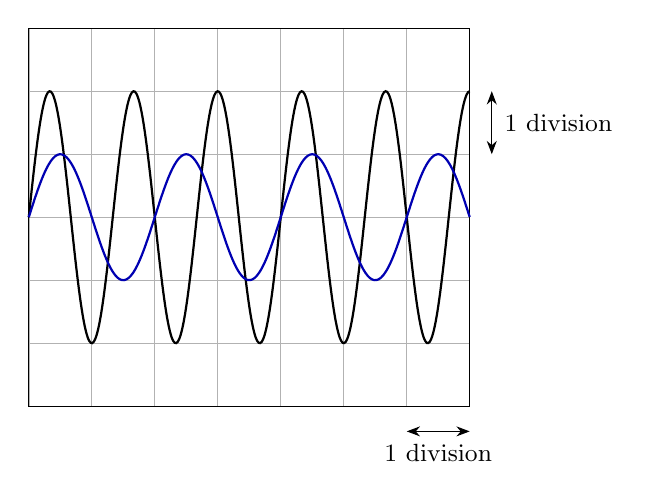
\begin{tikzpicture}[>=Stealth, font=\small, scale=0.8]
  % c.r.o. screen grid (7 by 6 divisions), centre line at y = 0
  \fill[white] (0,-3) rectangle (7,3);
  \draw[gray!60, very thin] (0,-3) grid (7,3);
  \draw (0,-3) rectangle (7,3);
  % given trace: amplitude 2 divisions, 3 waves in 4 divisions
  \draw[thick, domain=0:7, samples=300, smooth] plot (\x, {2*sin(270*\x)});
  % answer: smaller amplitude and longer period (lower frequency)
  \draw[blue!70!black, thick, domain=0:7, samples=200, smooth] plot (\x, {sin(180*\x)});
  \draw[<->] (7.35,1) -- (7.35,2);
  \node[right] at (7.4,1.5) {1 division};
  \draw[<->] (6,-3.4) -- (7,-3.4);
  \node[below] at (6.5,-3.45) {1 division};
\end{tikzpicture}
\end{center}
\end{ansbox}

%=================================================================
\examq{5054/22/M/J/16}{11}{The Nuclear Atom \textperiodcentered\ Radioactivity \textperiodcentered\ The Stars \& Universe}{15}

\begin{mstab}{q1color}
11(a) & (nucleus\,/\,nuclide\,/\,atom) with same number of protons & B1 \\ \hline
11(b)(i) & 2 & B1 \\ \hline
11(b)(ii) & neutron & B1 \\ \hline
11(b)(iii) & 2 & B1 \\ \hline
11(b)(iv) & 4 & B1 \\ \hline
 & nuclei repel\newline or like\,/\,positive charges repel & B1 \\ \cline{2-3}
\multirow{-2}{1.9cm}{11(c)} & (needs) high kinetic energy\,/\,speed (to overcome repulsion) & B1 \\ \hline
11(d) & ANY 3 lines from\newline $\bullet$ (dust\,/\,gas) collapses\,/\,comes together\,/\,clusters\,/\,condenses\newline $\bullet$ gravitational attraction or gravity mentioned\newline $\bullet$ temperature rises or KE (dust\,/\,gas) increases\newline $\bullet$ (nuclear) fusion occurs\newline $\bullet$ equilibrium established as radiation pressure\,/\,outward force balances inward force & B3 \\ \hline
 & time for a quantity to halve & C1 \\ \cline{2-3}
\multirow{-2}{1.9cm}{11(e)(i)} & time for (radio)activity\,/\,count rate\,/\,number of atoms\,/\,number of nuclei to halve & A1 \\ \hline
 & any relevant halving seen, e.g.\ $16\,000/2$ & C1 \\ \cline{2-3}
\multirow{-2}{1.9cm}{11(e)(ii)} & 1000 & A1 \\ \hline
\end{mstab}

\begin{ansbox}{q1color}
For (a), isotopes of hydrogen are \textbf{nuclei (atoms) of hydrogen that have the same number of protons} -- proton number $1$, which is what makes them all hydrogen -- but \textbf{different numbers of neutrons}, and therefore different nucleon numbers. The two in Fig.\,11.1 are $^{2}_{1}\mathrm{H}$ (one proton, one neutron) and $^{3}_{1}\mathrm{H}$ (one proton, two neutrons). Because the proton number fixes the number of electrons, isotopes of the same element are chemically identical; only their masses and nuclear stability differ.

For (b)(i), in the symbol $^{3}_{1}\mathrm{H}$ the lower number is the proton number and the upper number is the nucleon number, so
\[ \text{number of neutrons} = 3 - 1 = 2. \]

For (b)(ii), both nucleon number and proton number are conserved in the reaction. Adding up the left-hand side:
\[ \text{nucleons: } 2 + 3 = 5, \qquad \text{protons: } 1 + 1 = 2. \]
Particle B turns out to be $^{4}_{2}\mathrm{He}$ (see (iii) and (iv)), which accounts for $4$ of the $5$ nucleons and both protons. Particle A is therefore left with $1$ nucleon and $0$ protons -- it is a \textbf{neutron}, $^{1}_{0}\mathrm{n}$.

For (b)(iii), the two protons on the left must both end up in particle B, since the neutron A carries none, so the \textbf{proton number of B is $2$} (it is a helium nucleus).

For (b)(iv), of the $5$ nucleons on the left, $1$ goes to the neutron A, so B has
\[ 5 - 1 = 4 \ \text{nucleons}. \]
The \textbf{nucleon number of B is $4$}, confirming B as $^{4}_{2}\mathrm{He}$ -- an alpha particle. The complete equation is
\[ ^{2}_{1}\mathrm{H} + ^{3}_{1}\mathrm{H} \rightarrow\ ^{4}_{2}\mathrm{He} + ^{1}_{0}\mathrm{n}. \]

For (c), every nucleus carries a \emph{positive} charge, so as two nuclei approach each other \textbf{they repel} -- like (positive) charges repel -- and the electrostatic repulsion grows rapidly as the separation shrinks. Fusion can only happen if the nuclei get close enough for the very short-range \emph{strong nuclear force} to take over and bind them, which means they must \textbf{approach with enough kinetic energy (high enough speed) to overcome that repulsion}. Temperature is a measure of the average kinetic energy of the particles, so an extremely \textbf{high temperature} is what supplies the necessary speeds.

For (d), any \textbf{three} of the following stages earn the three marks:

\begin{itemize}[nosep,leftmargin=*]
\item \textbf{Gravitational attraction} acts between all the particles of the cloud, pulling them together.
\item The cloud of \textbf{gas and dust therefore collapses} -- it comes together, clusters and condenses into a much denser, smaller ball.
\item As it contracts, gravitational potential energy is converted to kinetic energy of the particles, so the \textbf{kinetic energy increases and the temperature rises} enormously.
\item Once the core is hot enough (millions of kelvin), the nuclei move fast enough to overcome their repulsion and \textbf{nuclear fusion of hydrogen begins}, releasing energy.
\item The star then becomes stable: an \textbf{equilibrium} is reached in which the \textbf{outward radiation pressure from the fusion balances the inward gravitational force}, so the star stops collapsing and shines steadily.
\end{itemize}

For (e)(i), the two marks are for the halving idea and for naming what halves. \textbf{Half-life is the time taken for a quantity to fall to half its value} -- specifically the time for the \textbf{activity (count rate), or the number of undecayed atoms or nuclei, of the sample to halve}. Saying only ``the time for something to halve'' is incomplete; saying ``the time for the sample to halve'' is wrong, since the mass does not change.

For (e)(ii), compare the elapsed time with the half-life:
\[ \text{number of half-lives} = \frac{48}{12} = 4. \]
Then halve the number of atoms four times:
\[ 16\,000 \xrightarrow{\ 12\ \mathrm{y}\ } 8000 \xrightarrow{\ 12\ \mathrm{y}\ } 4000 \xrightarrow{\ 12\ \mathrm{y}\ } 2000 \xrightarrow{\ 12\ \mathrm{y}\ } 1000. \]
So \textbf{$1000$ atoms} of $^{3}_{1}\mathrm{H}$ remain. Equivalently, $16\,000 \times \left(\tfrac{1}{2}\right)^{4} = 16\,000/16 = 1000$.
\end{ansbox}

\end{document}
